\chapter{Error control in ADS-B} \label{chap:adsb_parity}

In almost all digital telecommunications, error control is an essential capability. An adequate error control coding scheme in telecommunication allows a receiver to validate the correctness of the information that has been transmitted. Sometimes, it also provides the receiver with the ability to correct errors. Depending on the characteristics of the communication channel and the types of messages, different error control coding schemes can be adopted.

For error detection, three types of error control codes are broadly used, which are 1) parity, 2) checksum, and 3) cyclic redundancy check (CRC)\cite{grami2015}. Though there are similarities among these concepts, they should not be confused:

\begin{itemize}

 \item Parity is the simplest form of error detection. Commonly, the message is divided into segments of equal length. One parity bit is added to each segment and sent along with the message. The parity bit ensures either an even or odd number of \1 bits are contained in the segment. It guarantees the detection of at least one-bit errors. A two-dimensional parity check is also common, where additional parity bits are added to the same n-th bit in the segments.

 \item Checksum bits are longer and computed differently. The message is also first divided into segments of equal length. The checksum is generated by adding the segments using the \emph{ones' complements arithmetic} and sent along with the message. At the receiving side, the same arithmetic can be applied, where the complement of the sum should be zero.

 \item CRC is an algorithm based on binary polynomial arithmetic. A pre-defined divisor (also known as \emph{generator}) is used to compute the remainder using the binary polynomial division. The CRC remainder is appended to the message. The receiving side can run the same process on the entire message to check whether the remainder is zero. CRC is a much stronger method for error detection. It also offers the ability to correct errors \cite{mandel2009}.

\end{itemize}

\begin{notebox}{Note}
The CRC \emph{remainder} term is confusingly defined in Mode~S literature and standards. Many documents refer it as \emph{parity} or \emph{checksum}. To be consistent with Mode~S standards, such as \cite{icao9871v1, rtca2011mops}, parity, checksum, and CRC remainder are considered to be synonyms in this book. They all refer to the CRC remainder.
\end{notebox}

\section{CRC error control}

In Mode~S communications (including ADS-B), CRC error control coding is used. In all types of Mode~S downlink messages, the last 24 bits are reserved for the CRC remainder. In ADS-B, the CRC remainder is directly appended as the final 24 bits of the messages. However, in other types of Mode~S messages, those bits can be overlaid with other information (such as the ICAO address) using the \texttt{XOR} (\emph{exclusive disjunction}) operator before being appended to the message.

A basic CRC workflow is shown in Figure \ref{fig:crc_flow}. The diagram on the left-hand side shows how the CRC remainder is generated on the sender side. The diagram on the right-hand side shows how the same arithmetic can be used on the receiver side to validate the message.

\begin{figure}[ht]
  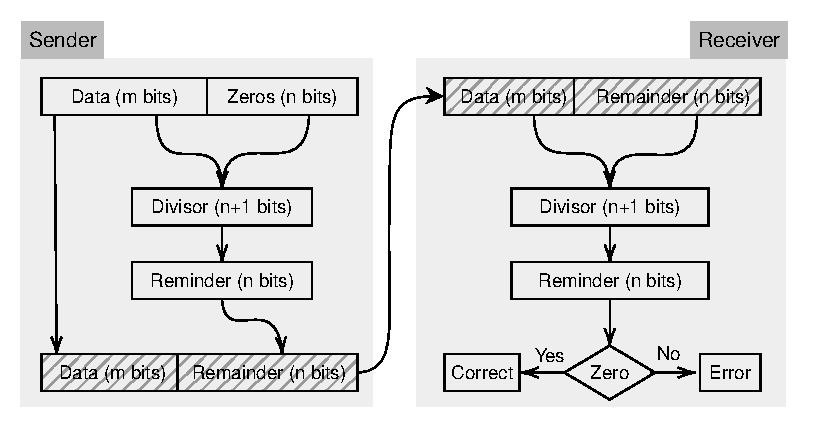
\includegraphics[scale=0.9]{figures/crc/crc_flow.pdf}
  \caption{The CRC error control processes}
  \label{fig:crc_flow}
\end{figure}


The binary polynomial falls in the finite field arithmetic \cite{carlitz1932}. The divisions of binary polynomials can essentially be considered as the \texttt{XOR} bitwise operations, which can be easily implemented and calculated by computers. In Figure \ref{fig:crc_example}, a CRC remainder calculation example is shown.



\begin{figure}[ht]
  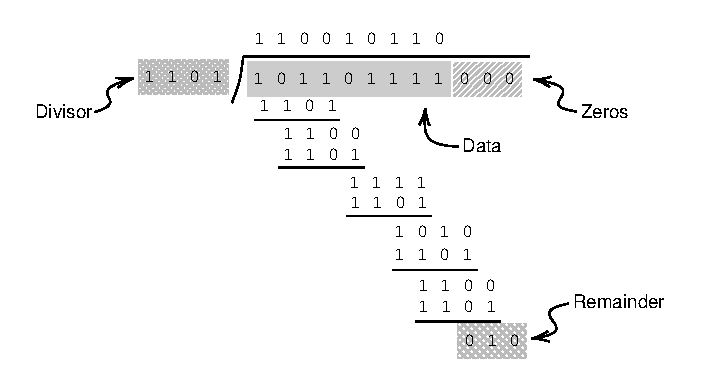
\includegraphics[scale=0.9]{figures/crc/crc_example.pdf}
  \caption{A CRC example with a 4-bit divisor and 3-bit remainder}
  \label{fig:crc_example}
\end{figure}


\section{ADS-B parity}

The polynomial form of the divisor (generator) used for ADS-B (as well as other Mode~S messages) is shown as following \cite{gertz1984}:

\begin{equation}
  \begin{split}
  G(x) = &x^{24}+x^{23}+x^{22}+x^{21}+x^{20}+x^{19}+x^{18}+x^{17} \\
         &+x^{16}+x^{15}+x^{14}+x^{13}+x^{12}+x^{10}+x^{3}+1
  \end{split}
\end{equation}

where $G(x)$ represents the generator function. This generator code was found by \cite{kasami1964}, which is known for its efficiency to correct burst errors. A 24-bit remainder is generated using this generator. It can also be written in different formats as:

\begin{verbatim}
Binary:   1111111111111010000001001
Decimal:  33551369
Octal:    177772011
HEX:      1FFF409
\end{verbatim}

Knowing the logic of CRC, the computation of the remainder and the verification of error is fairly simple. Let  $x^{i}$ represent each bit of the message and $M(x)$ represent the polynomial corresponding ADS-B message, the CRC remainder (parity) $P(x)$ can thus be calculated as:

\begin{equation}
  \begin{split}
    M(x) &= \sum_{i=0}^{87} a_i x^i , \quad a_i \in (0, 1)\\
    P(x) &= M(x) ~ \% ~ G(x)
  \end{split}
\end{equation}

In the following pseudocode, the algorithm for computing the remainder of an ADS-B message is shown:

\begin{verbatim}
generator = 1111111111111010000001001

data_hex = 8D406B902015A678D4D220[000000]     # 11 + 3 zero bytes

data = 1000110101000000011010                 # 88 bits
       1110010000001000000001
       0101101001100111100011
       0101001101001000100000
      [000000000000000000000000]              # append 24 zero bits

FOR i FROM 0 TO (112-24):
  IF data[i] IS 1:
    data[i:i+24] = data[i:i+24] XOR generator

remainder = data[-24:]

# final result: 101010100100101111011010, or AA4BDA in hexadecimal
\end{verbatim}

To check whether an error occurs in the message, replace the \texttt{data\_hex} in the previous example with the received message and run the same CRC process. The message is correct if all final 24 remainder bits are zeros.

\begin{notebox}{Try it out}
Using \texttt{pyModeS}, we can check the correctness of a ADS-B message as: 

\begin{verbatim}
import pyModeS as pms

msgA = "8D406B902015A678D4D220AA4BDA"
msgB = "8D4CA251204994B1C36E60A5343D"

remainderA = pms.crc(msgA)  # should be 0
remainderB = pms.crc(msgB)  # should be 16
\end{verbatim}

When the remainder is zero, the message is not corrupted. Otherwise, the error has occurred during the transmission.
\end{notebox}